\chapter{表格与图片管理}

% =========================================================
\section{基础表格 (tabular) 与三线表 (booktabs)}

在 \LaTeX{} 中，排版表格主要使用 \texttt{tabular} 环境。三线表通过 \texttt{booktabs} 宏包提供的水平线提升专业感。

\begin{lstlisting}[language={[LaTeX]TeX}, caption={三线表源码}, frame=single]
\begin{table}[H]
    \centering
    \caption{三线表样式演示}
    \begin{tabular}{ccc}
        \toprule
        \textbf{实验组} & \textbf{参数 A} & \textbf{结果 B} \\
        \midrule
        Control        & 1.00           & 0.85           \\
        \bottomrule
    \end{tabular}
\end{table}
\end{lstlisting}

\begin{table}[H]
    \centering
    \caption{三线表样式演示}
    \begin{tabular}{ccc}
        \toprule
        \textbf{实验组} & \textbf{参数 A} & \textbf{结果 B} \\
        \midrule
        Control        & 1.00           & 0.85           \\
        Group 1        & 2.50           & 1.12           \\
        Group 2        & 5.00           & 2.04           \\
        \bottomrule
    \end{tabular}
\end{table}

TexStudio中有关于直接插入表格的按钮，但我更喜欢用https://www.latex-tables.com/，可以直接把表格转换成\LaTeX 代码，很方便。
\section{图片插入与路径管理}

图片插入的核心命令是 \texttt{\textbackslash includegraphics}。建议将图片统一放在 \texttt{Figure/} 文件夹下。

\begin{figure}[H]
    \centering
    % 如果没有实际图片，编译时请确保路径正确或使用 draft 模式
    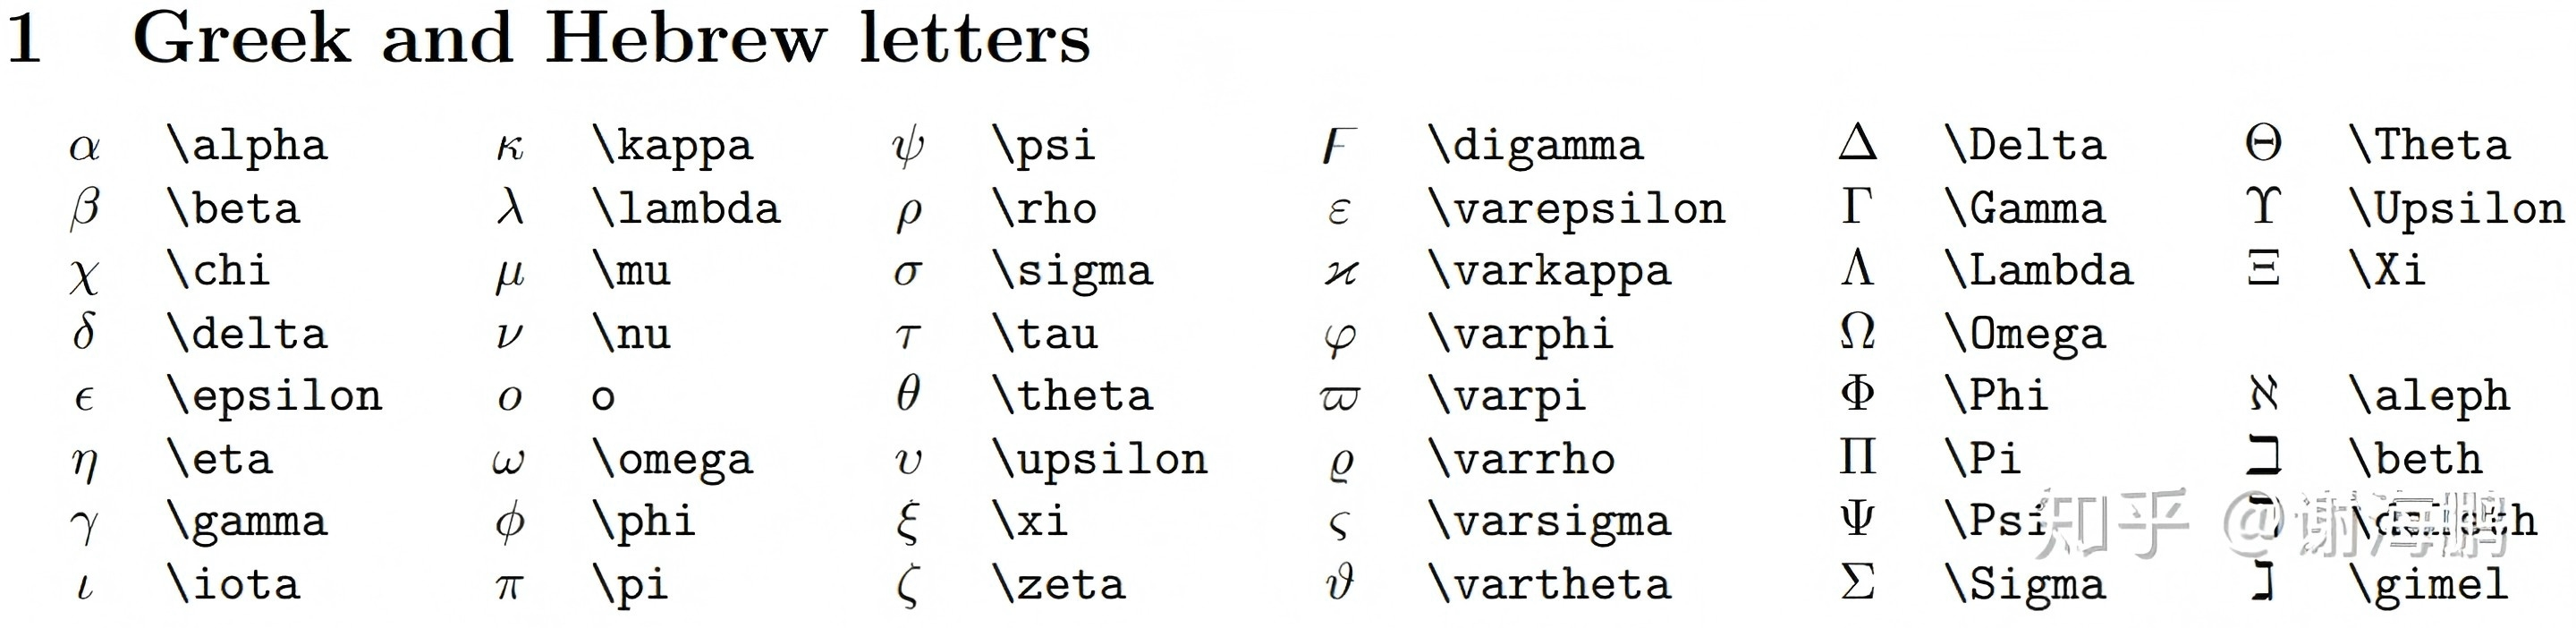
\includegraphics[width=0.6\textwidth]{Figure/1.jpg} 
    \caption{这是你的第一张独立图片} 
\end{figure}



\section{浮动体 (Float) 原理}

\begin{itemize}
    \item \texttt{[h]}: 尽量放在当前处。
    \item \texttt{[H]}: 强制固定（需 \texttt{float} 宏包），适合对位置要求极高的逻辑推导。
\end{itemize}

\begin{tcolorbox}[colback=blue!5, colframe=blue!50, title=排版建议]
    若编译时间过长，可在 \texttt{\textbackslash documentclass} 中临时开启 \texttt{draft} 选项，跳过图片渲染。
\end{tcolorbox}